\begin{savequote}[75mm]
Some Quote.
\qauthor{Quoteauthor Lastname}
\end{savequote}

%For an example of a full page figure, see Fig.~\ref{fig:myFullPageFigure}.

\chapter{Introduction}
\newthought{There's something to be said} for having a good opening line.
\section{Problem Definition and Motivation}
This chapter presents the motivation behind our work by first discussing the three underlying problems that will be addressed throughout. To summarize into a brief statement, we would say our overall goal is the decomposition of video into semantically meaningful entities. That is, to move from the base \emph{low-level} pixels which compose an image to \emph{high-level} structures which are more representative of how a human would understand the scene. In the following sections we will introduce the three constituent underlying sub-problems: Image Segmentation, Multi-Target Tracking, and Video Object Segmentation.

\todo[inline]{Motivation, put some applications}

\subsection{The Image Segmentation Problem}
Image segmentation aims to divide the set of pixels in an image into a number of distinct subsets, where each subset represents some semantically meaningful entity (e.g., an object - see Fig. \ref{fig:segmentation_example}). This is a notoriously tricky business, particularly because it is something that humans are able to do intuitively. This ease with which humans can segment visual scenes is highly deceptive; Marvin Minsky, one of the pioneers of Artificial Intelligence (AI), famously assigned one of his students ``computer vision'' as a summer undergraduate project in 1966. Nearly half a century later, despite the extensive effort to solve it, image segmentation, the first step on the long road to complete ``computer vision'', remains an unsolved problem. 

\todo[inline]{Some citations about image segmentation by humans (from CVPR paper)}
\begin{figure}
\label{fig:SegmentationExample}
\centering
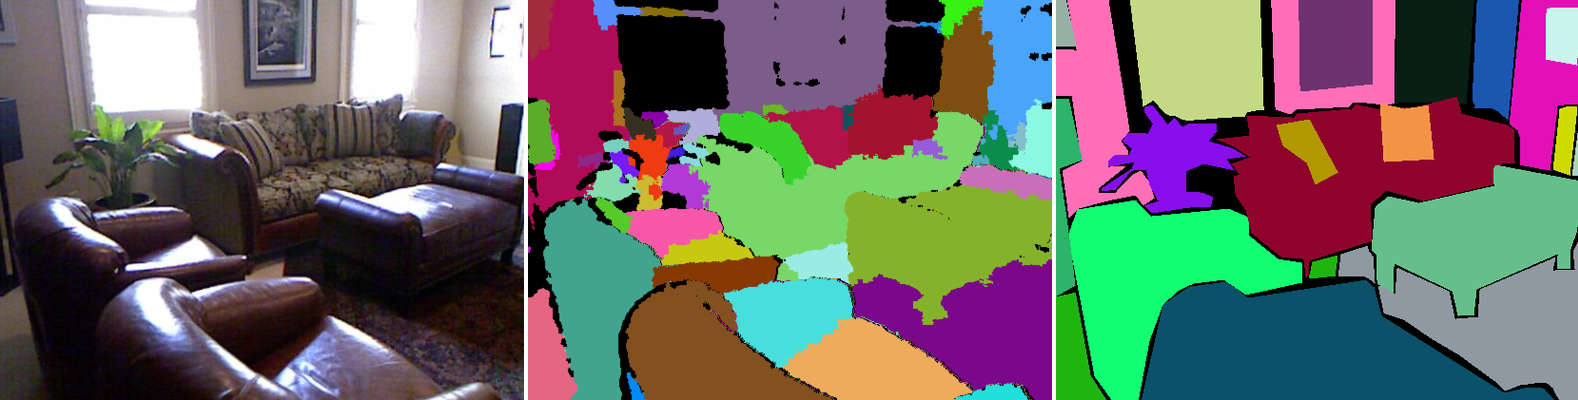
\includegraphics[width=\linewidth]{figures/Introduction/segmentation_GT_example.png}
\caption[Example of Segmentation and Ground Truth]{Example of Segmentation and Ground Truth. From left to right we have an image, a segmentation from a computer vision algorithm, and a human-annotated ground truth labeling. Here labels are represented by different colors. We shall use this convention throughout the rest of this work.}
\end{figure}

The reason for this is two-fold: firstly, there are many technical or physical challenges associated with properly dividing an image into separate objects. Among these, shadows, occlusions, reflections, imaging noise and so forth can all greatly affect the results of image segmentation. Consider, for instance, a partial occlusion as in Fig. \ref{fig:SegmentationProblems}. A human can easily identify that the parts on either side of the occluder belong to same object. This is accomplished using what we shall refer to as \emph{high-level} knowledge throughout this work - in this case, knowledge of the complete nature of an object. 

This leads us to the second challenge in image segmentation, which is that, generally speaking, there is no ``correct'' solution to the problem. A perfect labeling for one application might be useless in another. This is even more of a problem when we are discussing segmentation separate from any application, as is the case with standard image segmentation benchmarks (which are use to quantify algorithm performance). These benchmarks use ground-truth image labels (manually created by humans) to score the output of different algorithms. Unfortunately, the correctness of different labelings is highly subjective, and hand-drawn labels from  people can differ radically.

\begin{figure}
\label{fig:SegmentationProblems}
\centering
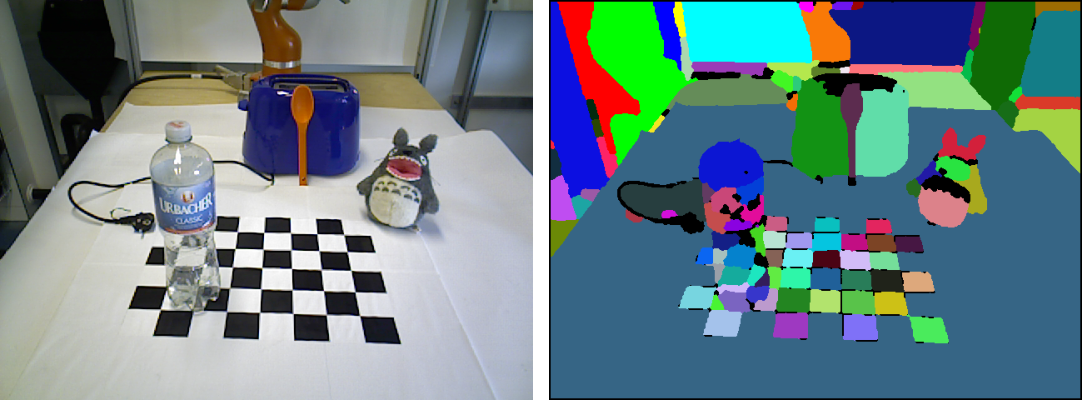
\includegraphics[width=\linewidth]{figures/Introduction/Segmentation_Problems.pdf}
\caption[Technical Difficulties of Segmentation]{Technical Difficulties of Segmentation. Here we see some of the myriad of technical difficulties present in color-based segmentation, such as transparent objects (the water bottle), partial occlusions (the toaster), objects with strong color differences (the little monster), and similarities in color (the bottle cap to the table).}
\end{figure}


\subsection{The Tracking Problem}
Multi-target visual tracking (MTVT) is a crucial challenge for many computer vision applications such as visual surveillance, action recognition, and robotic imitation learning. In many such functions, visual tracking serves as the precursor to all further high-level inference, making robust tracking fundamental to the success of a large variety of intelligent systems. The general goal of MTVT is to sequentially estimate the number of targets and their corresponding states (e.g., position, velocity). This is accomplished by associating noisy observations over time with the entities which produced them. Tracking links targets into sequential states (known as \emph{tracks}), typically using some a-priori detection model, such as tracking a human face in video based on a facial model. In general, this is done by estimating some state for each tracked object (e.g. a bounding box around a person's face) given an observation (e.g., the output of a face detector).

\begin{figure}
\label{fig:ExampleTracking}
\centering
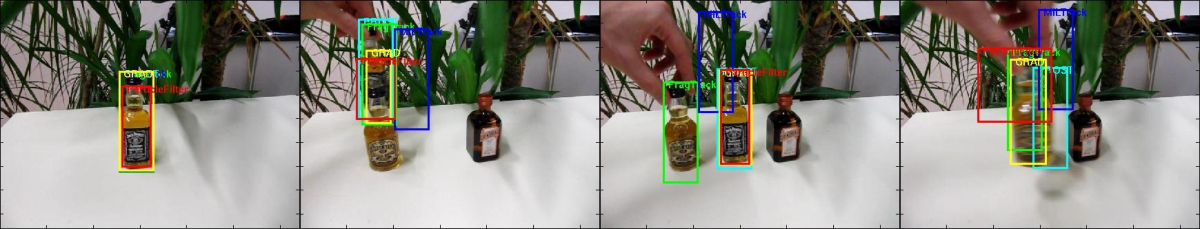
\includegraphics[width=\linewidth]{figures/Introduction/Tracking_Example.pdf}
\caption[Example of Visual Tracking]{Example of Visual Tracking. This shows outputs from various trackers in a standard video tracking benchmark. Some of the difficulties of tracking can be seen- in particular complex backgrounds, motion blur, partial occlusions (second frame from left) and even full occlusions (right-most frame).}
\end{figure}

The primary challenge in MTVT is the data association problem - deciding which tracked target a particular observation belongs to. Confounding this is the additional null possibility, where an observation belongs to none of the tracked targets. Closer examination reveals that the difficulties are related to those of image segmentation, simply extended into the temporal dimension. In particular, interacting and occluded targets are especially challenging.

\subsection{Video Object Segmentation - Segmentation In Sequential Frames}
Video object segmentation (VOS) attempts to cluster pixels of video frames into segments which are both spatially and temporally coherent. While similar to MTVT, VOS goes a step beyond localizing tracked objects, in that it makes an association decision for each observed pixel; in addition to estimating overall state, it must re-estimate spatial extent every frame. Additionally, VOS has the additional consideration that target appearance models are unknown a-priori, and are subject to arbitrary changes over time. 

\begin{figure}
\label{fig:ExampleSegmentation}
\centering
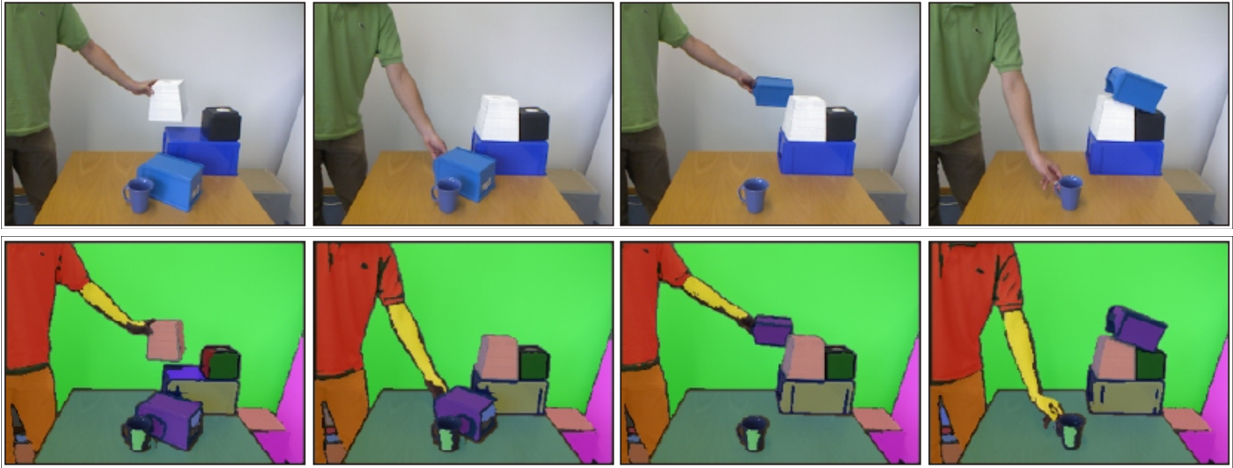
\includegraphics[width=\linewidth]{figures/Introduction/Video_Segmentation.pdf}
\caption[Example of Video Object Segmentation]{Example of Video Object Segmentation - from \cite{Abramov_WACV12}. This shows the goal of VOS - to extract a dense labeling (labels here are shown as distinct colors) for every frame, maintaining temporal consistency of objects. For many applications it is of vital importance to make the labeling consistent from frame to frame, that is, to maintain object identities.}
\end{figure}

One interesting aspect of video segmentation is that it has the potential to be more accurate than single image segmentation, as it can take advantage of the temporal coherence of objects to infer information about the objects in a scene. Unfortunately, the addition of the temporal domain brings along new challenges as well; for instance that pixels which should be grouped across time may not be continuously visible, as in the case of partial or full occlusions. Additionally, the added dimension increases the computational complexity of the problem, making accurate segmentation a costly procedure. Temporal information also increases the exposure of the algorithm to noise, as each image frame is a separate noisy measurement. This adds a large amount of uncertainty to the problem, since measured values (i.e., of color) for an object can show significant variation over time. 
 
\section{State of the Art}
\subsection{Segmentation and Superpixels}
Segmentation of scenes into objects remains one of the most challenging topics of computer vision despite decades of research. To address this, recent methods often use hierarchies which create a rank order that build bottom-up from small localized superpixels to large-scale regions \cite{Ren:ICCV2003,Ahuja:CVPR2008,Arbelaez:PAMI2011}. As an alternative, researchers have also pursued strictly top-down approaches. Such methods began with coarse segmentations using multiscale sliding window detectors \cite{ViolaJones:IJCV2004}, later progressing to finer grained segmentations and detections based on object parts \cite{Felzenswalb:PAMI2010, Bourdev:ICCV2009}. These two avenues of research led naturally to methods which {\em combine} bottom-up hierarchy building with top-down object- and part-detectors \cite{Arbelaez:CVPR2012, Silberman:ECCV12, Gupta:CVPR2013}. While these approaches have yielded quite good results even on complex, varied data sets, they have lost much of the generality of learning-free approaches. In general the most powerful methods to-date use trained classifiers for segmentation \cite{Silberman:ECCV12, Gupta:CVPR2013}. This means they cannot be applied to arbitrary unknown scenes without being retrained, requiring the acquisition of a new data-set tailored to each test environment.

\subsection{Multi-Target Visual Tracking}
Multi-Target Visual Tracking is a well-established field, which goes back over thirty years \cite{MTT_JPDA}. In this work we use Sequential Bayesian Filtering (SBF), a technique which recursively estimates the time-changing posterior distribution of target states given all previous observations. We use a Sequential Monte Carlo method known as Particle Filtering to approximate the posterior, an approach which was first introduced to the vision community by Isard and Blake \cite{Condensation98} and has been the subject of much subsequent research extending it to multiple targets \cite{TrackingMultipleParticleFiltering,MonteCarloMTT,SequentialMonteCarloMultitargetFiltering}. For details on how one approximates SBF using a Particle Filter we refer the reader to Appendix B.

Initially, researchers pursued two avenues of research in extending a single Particle Filter to multiple targets. The first was to represent all targets jointly in a single particle filter by assigning individual particles to particular labels \cite{MultiMixtureTracking03}. This means that, for a given total number of particles, there will be fewer for each individual target - resulting in reduced accuracy. The second approach was to add additional dimensions to the state space for each additional target \cite{TrackMultTargets01}. Unfortunately, this approach quickly increases the dimensionality of the state space, resulting in a need for a very high number of particles for the filter to remain accurate. In both approaches, the computational complexity increases exponentially as targets are added (for constant level of accuracy), as both seek to find a joint solution. As a consequence of this, it is beneficial to use a separate particle filter for each target. One way of doing this is to add factors to the observation and/or process models of the filters which explicitly model occlusions and interactions between targets \cite{MCMCParteFilt_05, ApproxMultiTrack_06}. 

Another approach which has generated much interest is to use the output of detectors as the basis for tracking. Known as \emph{tracking-by-detection}, these methods typically use independent particle filters to maintain tracks \cite{RobustVTMT_06,MultipersonTBD_011}, and place the focus of the problem on the data association step, wherein detections are assigned to targets. While there are several classical approaches for solving this association problem from Sonar and Radar research \cite{SonarMultiTrack_83,MultiTrack_79}, a greedy approach is typically sufficient given a good association scoring function \cite{DetTrackMultiHumans_07,MultipersonTBD_011}. 
%%%%%%%%%%%%
%Good review in - Detection and Tracking of Multiple, Partially Occluded Humans by Bayesian Combination of Edgelet based Part Detectors
%%%%%%%%%%%%%%%%%%%%%%%%%%%%

\subsection{Video Object Segmentation}
There are many existing video object segmentation (VOS) methods, which can be classified based on three parameters; whether they are on- or off-line, whether they are dense or sparse, and whether or not they are supervised. We can reduce the comparison-space of related work by comparing only with algorithms which have the same three parameters as this work - on-line processing (the algorithm may only use past data), dense segmentation (every pixel is assigned to a spatio-temporal cluster), and unsupervised operation. Four state-of-the-art segmentation algorithms meet these requirements: Mean-shift video segmentation (MSVS) \cite{MSVS}, Multiple hypothesis video segmentation (MHVS) from superpixel flows \cite{MHVS}, Propagation, validation, and aggregation (PVA) of a preceding graph \cite{PropValAgg}, and Matching images under unstable segmentations \cite{MatchingUnstable}.  Of these methods, none are able to handle full occlusions; in fact only MHVS considers occlusions, and it is only able to handle partial 
occlusions for a few frames, and does not consider full occlusions. Even state of the art off-line methods such as that of Brendel and Todorovic \cite{SegTrackRegions} only handle partial occlusions, claiming that ``complete occlusions ... require higher-level reasoning''.  

Multiple hypothesis video segmentation (MHVS) from superpixel flows \cite{MHVS} provides dense online unsupervised video segmentations, but is only able to handle partial occlusions for a few frames, and does not consider full occlusions. There also has been much recent work in VOS specifically addressing the problem of segmenting foreground from background \cite{MWCwMC,GC_SURF}. While these works have been to shown to perform very well in their task, they only solve the single target case, as they do not need to resolve the multiple association problem.

In \cite{TrackingOcclusionsGraphCuts} Papadakis and Bugeau use a dynamical model to guide successive segmentations, along with an energy function minimized using graph cuts to solve the label association problem. They formally model visible and occluded regions of tracked objects, tracking them as distinct parts. While they do consider occlusions, they do not maintain a world model, and as such their methodology must fail under complete occlusions.  Additionally, they formally model visible and occluded parts of the tracked objects, and so the method does not scale well with an increasing number of objects, and thus is better suited to extracting the silhouettes of a few objects than performing a full segmentation. Other methods, such as \cite{LayeredGraphicalModels}, are severely limited in that they require pre-
computed models which are calibrated to a ground plane in order to resolve occlusions. Recent work in MTVT~\cite{MultiObjectTracking} successfully tracks multiple objects using a segmentation and association approach and adaptive 3D appearance models, but is limited by the need to align model point clouds to the observed data every frame, as well as the need for a ground plane. This precludes it from handling occlusions, as once a target is no longer observed, its track must be terminated.

\section{Outline and Contributions}

This thesis is organized as follows: First, in Chapter \ref{Chap:VideoSegRelaxation} we present a hybrid Video Object Segmentation / Multi-Target Tracking technique for 2D data. We describe the method, briefly describe the segmentation algorithm it relies on, and present results on a tracking benchmark. In Chapter \ref{Chap:WorldModel} we present the concept of a persistent 3D voxel world model. We begin by briefly introducing some core concepts of acquisition and representation of 3D pointcloud data, then present Voxel Cloud Connectivity Segmentation (VCCS), a method for extracting a graph of 3D voxel patches from pointcloud data. We then discuss how to add pointclouds sequentially to the model in a way that allows voxels to persist through occlusions. In Chapter \ref{Chap:ModelBasedTracking} we describe a method for using particle filters to track multiple rigid objects in pointcloud video data and present results of tracking performance on artificial data. In Chapter \ref{Chap:TrackingBasedSegmentation} we combine the methods described in prior Chapters into a system which can produce full video segmentation of pointcloud videos. We show that the system is highly robust to occlusions and noisy data, and give results for the application of semantic understanding of human actions. Finally, in Chapter \ref{Chap:Conclusions} we discuss the findings and experimental results of this work, possible future work, and conclude.

Each of the Chapters in this thesis contain novel contributions to the field: Chapter \ref{Chap:VideoSegRelaxation} contains the 2D segmentation through relaxation technique. Chapter \ref{Chap:WorldModel} contains the Supervoxel clustering method, as well as the scheme for maintain voxels in an Octree through occlusions. Chapter \ref{Chap:ModelBasedTracking} has the scheme for accelerating 3D particle filter tracking through stratified sampling of the model-space. Finally, Chapter \ref{Chap:TrackingBasedSegmentation} has the techniques used to generate full segmentations based upon the results from multiple independent trackers. Additionally, Appendix A presents the Oculus Vision System, a computer vision system created over the course of the research for this thesis.